\section{Introduzione}



\textcolor{blue}{\lipsum[1]}

\section{Background}

\textcolor{blue}{\lipsum[1-4]}

\begin{figure}[t!]
	\centering
	\footnotesize{
	 \def\svgwidth{\linewidth}
	 \input{rheometer.pdf_tex}}
	\caption{}
	\label{fig:system}
\end{figure}


\begin{figure*}[h!]
	\begin{subfigure}{0.5\linewidth}
	\centering
	\footnotesize{
	\def\svgwidth{0.9\linewidth}
	\input{mechanic_model.pdf_tex}}
\caption{}
\label{fig:mechanical}
	\end{subfigure}\hfill
	\begin{subfigure}{0.5\linewidth}
	\centering
	\footnotesize{
	\def\svgwidth{0.9\linewidth}
	\input{creep_response.pdf_tex}}
\caption{}
\label{fig:mechanical1}
\end{subfigure}\hfill
\caption{text}
\end{figure*}



\subsection{Microreometro a biglia magnetica}




\section{Risultati}

\begin{figure*}[t!]
\begin{lstlisting}[language=matlab]
	function dydt=zener_displacement(t,y,parameters,tspan,flag)
		k_0=parameters(1);
		k_1=parameters(2);
		gamma_0=parameters(3);
		gamma_1=parameters(4);
		F_bar=parameters(5);
		switch flag
			case 'square'
				[F, dF]=force(t,tspan);
				dydt=((F-k_0*y)/gamma_1 + (dF/k_1))*(1+k_0/k_1);
			case 'step'
				dydt=(-(k_0/gamma_1)*y+(F_bar/gamma_1))/(1+(k_0/k_1));
			case 'harmonic'
				omega=parameters(7);
				F=F_bar*(1+sin(omega*t));
				dF=F_bar*omega*cos(omega*t);
				dydt=((F-k_0*y)/gamma_1 + (dF/k_1))*(1+k_0/k_1);
		end
	end
\end{lstlisting}
\caption{Routine richiamata da \texttt{ode15s} per la soluzione dell'equazione differenziale per lo spostamento del corpo Zener}
\vspace{0.8cm}
\begin{lstlisting}[language=matlab]
	function dydt=dashpot_displacement(t,y,parameters,tspan,flag)
		gamma_0=parameters(3);
		gamma_1=parameters(4);
		F_bar=parameters(5);
		switch flag
			case 'square'
				[F, dF]=force(t,tspan);
				dydt=F/gamma_0;
			case 'step'
				dydt=F_bar/gamma_0;
			case 'harmonic'
				omega=parameters(7);
				F=F_bar*(1+sin(omega.*t));
				dF=F_bar*omega*cos(omega*t);
				dydt=F/gamma_0;
		end
	end	
\end{lstlisting}
\caption{Routine richiamata da \texttt{ode15s} per la soluzione dell'equazione differenziale per lo spostamento dello smorzatore}
\end{figure*}


\begin{figure*}[t!]
	\begin{lstlisting}[language=matlab]
function [F, dF]=force(t_curr,t)	
	T_cyc=5;
	N_cyc=4;
	F=2000;
	freq=1/T_cyc;
	squareWave=F/2*(square(2*pi*freq*t,50)+1);
	squareWave(end)=0;
	squareWave_smooth=smoothdata(squareWave,'gaussian',(size(t)/N_cyc)*0.05);
	derivate=[0 diff(squareWave_smooth)];
	F=interp1(t,squareWave_smooth,t_curr);
	dF=interp1(t,derivate,t_curr);
end
	\end{lstlisting}
	\caption{Routine per la generazione dell'onda quadra regolarizzata di ingresso. Viene inserita anche la funzione \texttt{interp1} per permette a \texttt{ode15s} di leggere il valore di forza a qualsiasi instante temporale ($\mathtt{t\_curr}$) e non solo sui campione dove è stato definito il segnale.}
\end{figure*}

\begin{figure}[t!]
	\centering
	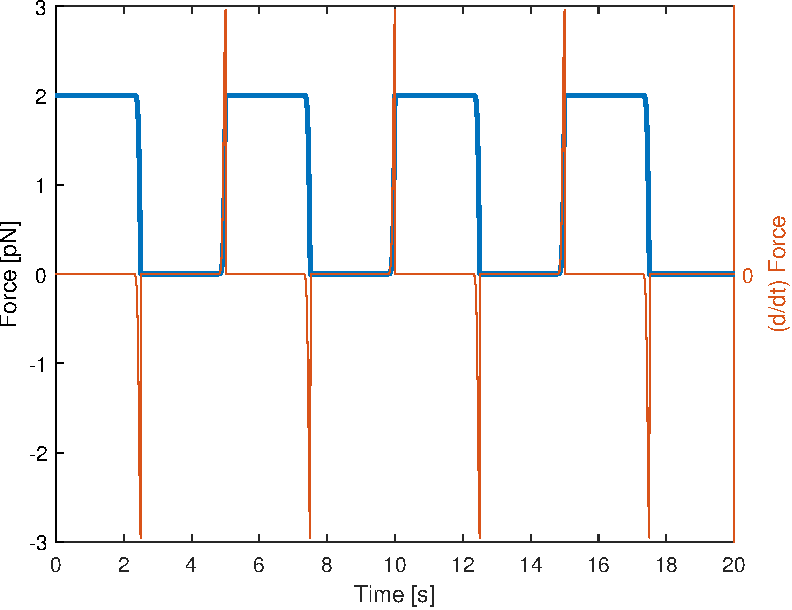
\includegraphics[width=0.95\linewidth]{../code/figs/square_regularized}
	\caption{}
	\label{fig:squareregularized}
\end{figure}



\begin{figure*}[t!]
	\begin{subfigure}{0.5\linewidth}
	\centering
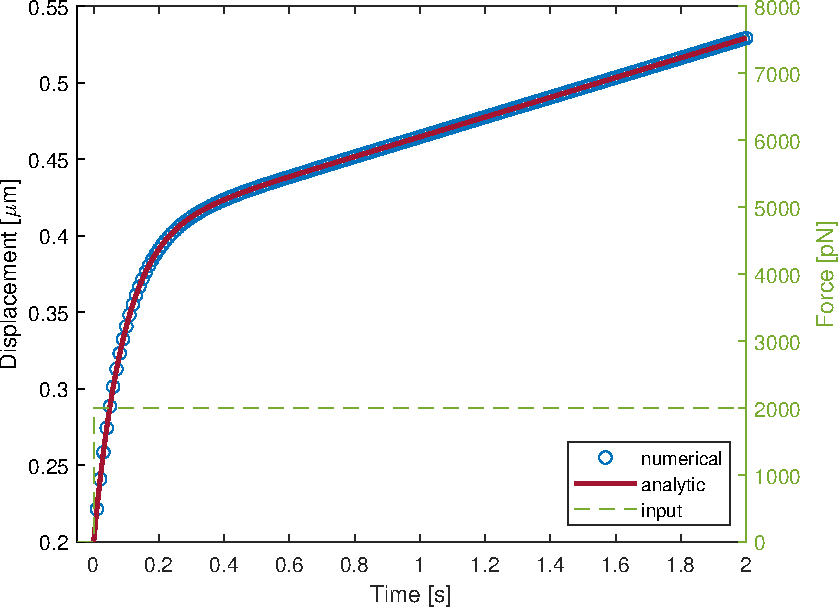
\includegraphics[width=0.95\linewidth]{../code/figs/step}
\caption{}
\label{fig:square}
	\end{subfigure}\hfill
	\begin{subfigure}{0.5\linewidth}
	\centering
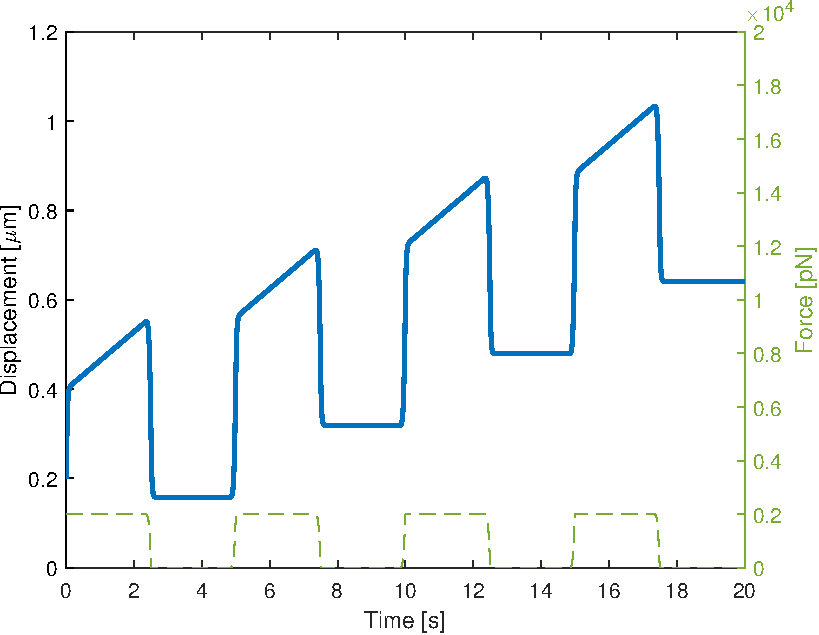
\includegraphics[width=0.95\linewidth]{../code/figs/square}
\caption{}
\label{fig:step}
\end{subfigure}\hfill
\caption{Risposta del sistema ad ingresso a gradino (a) e ad onda quadra con periodo di 5s (b).}
\end{figure*}

\begin{figure*}[t!]
	\centering
	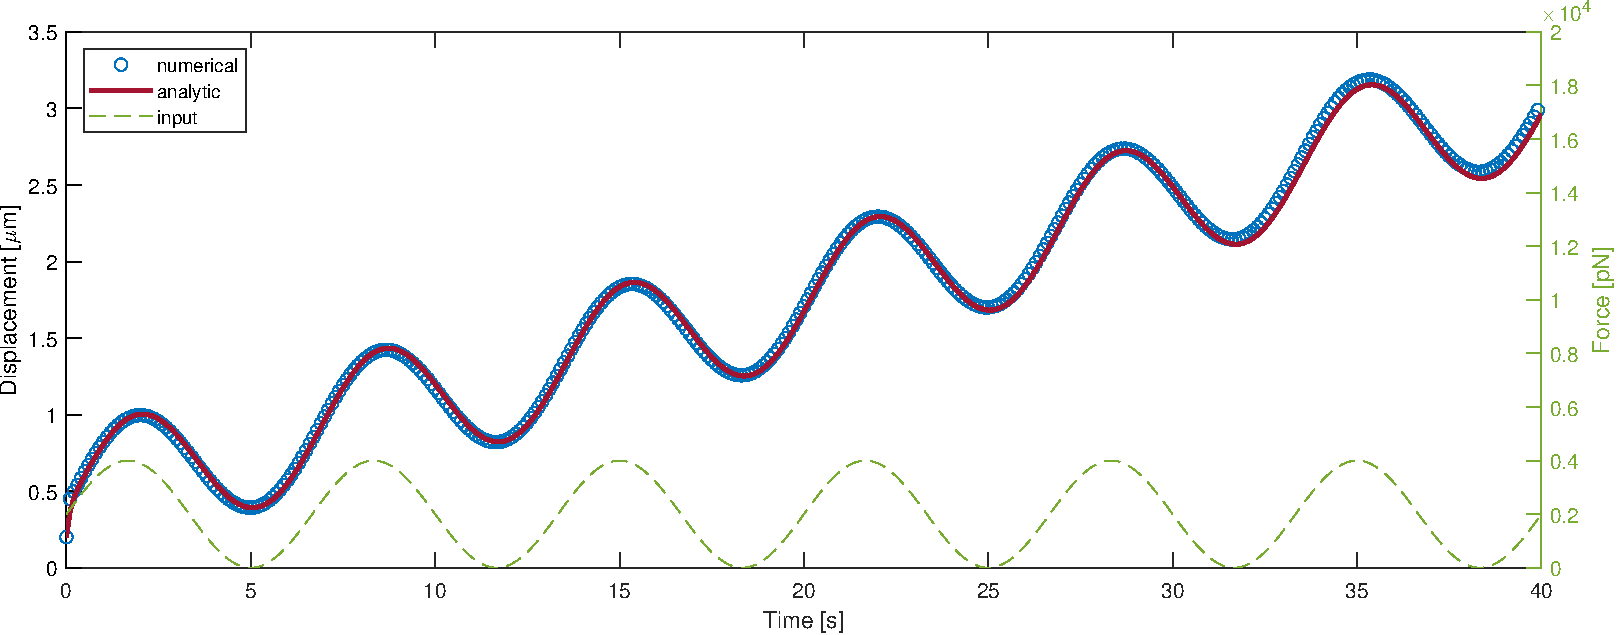
\includegraphics[width=0.95\linewidth]{../code/figs/harmoniclarge}
	\caption{Confronto tra il risultato analitico e il risultato numerico con ingresso sinusoidale a frequenza 0.15 Hz applicato per 40s.}
	\label{fig:harmoniclarge}
\end{figure*}

\begin{figure*}[t!]
	\begin{subfigure}{0.33\linewidth}
		\centering
			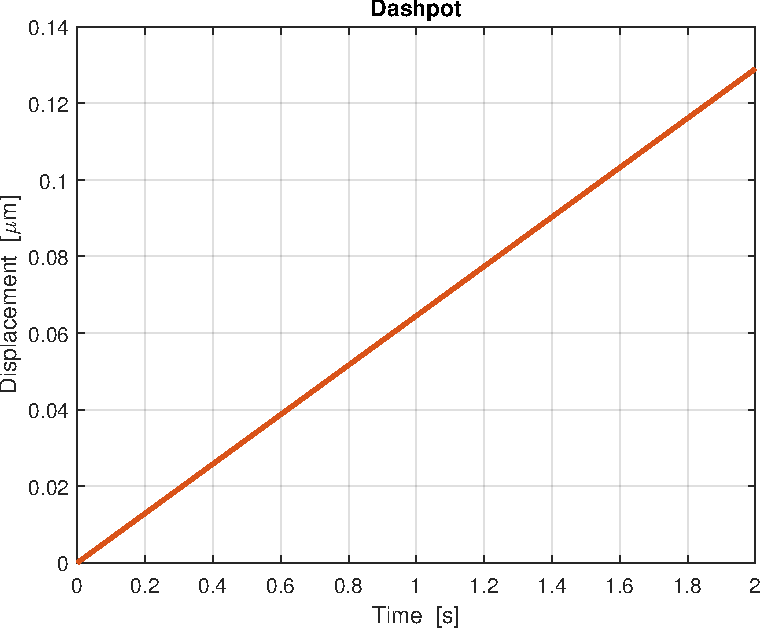
\includegraphics[width=0.95\linewidth]{../code/figs/step_dashpot_}
		\caption{}
	\end{subfigure}\hfill
	\begin{subfigure}{0.33\linewidth}
	\centering
		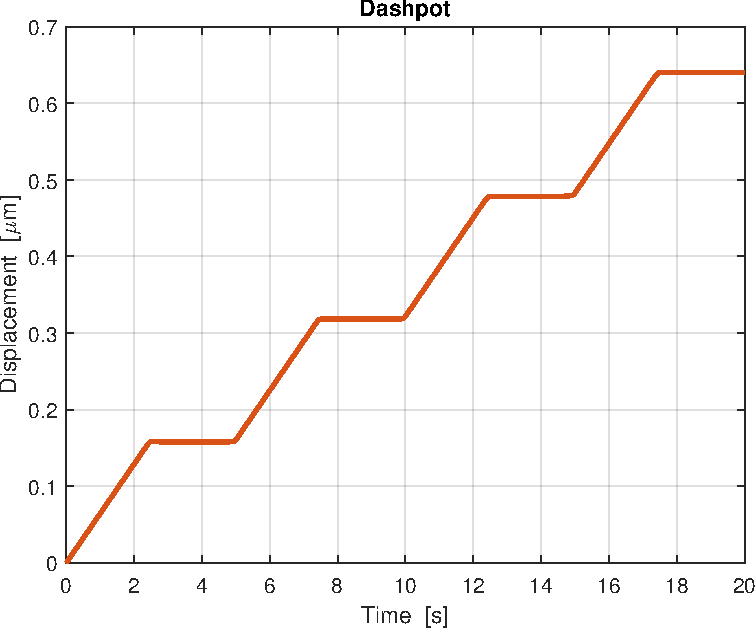
\includegraphics[width=0.95\linewidth]{../code/figs/square_dashpot_}
	\caption{}
\end{subfigure}\hfill
	\begin{subfigure}{0.33\linewidth}
	\centering
	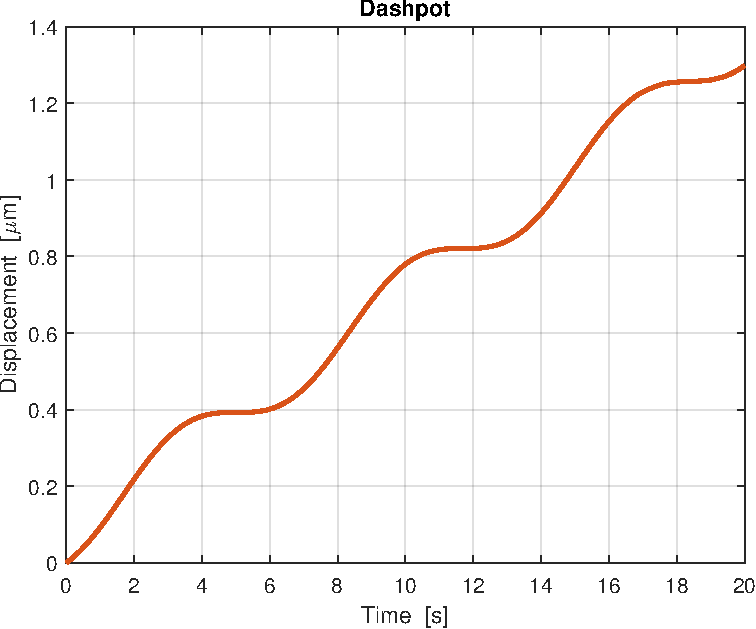
\includegraphics[width=0.95\linewidth]{../code/figs/harmonic_dashpot_}
	\caption{}
\end{subfigure}\hfill
	\begin{subfigure}{0.33\linewidth}
		\centering
			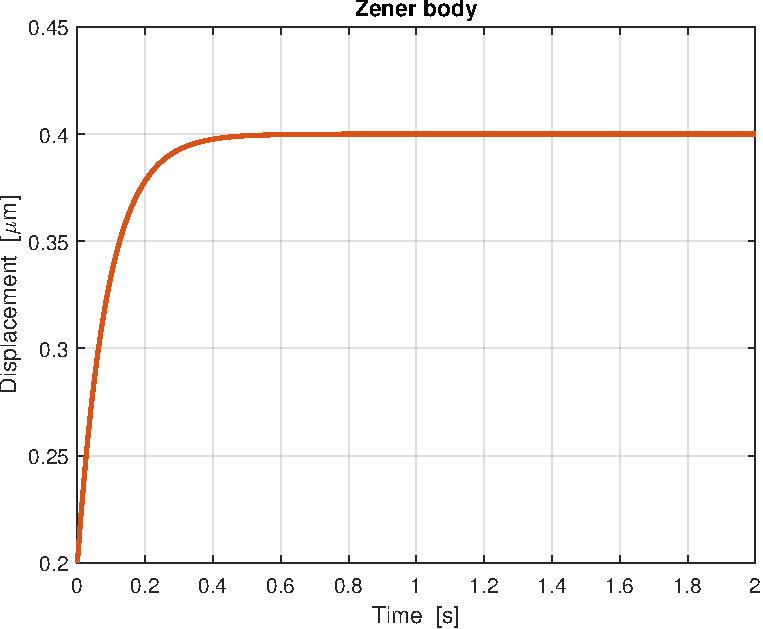
\includegraphics[width=0.95\linewidth]{../code/figs/step_zener_}
		\caption{}
	\end{subfigure}\hfill
	\begin{subfigure}{0.33\linewidth}
		\centering
		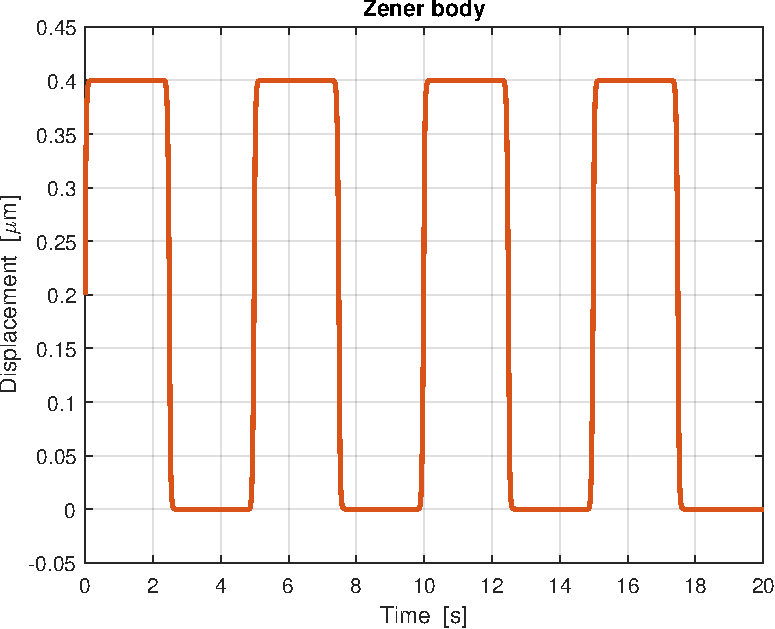
\includegraphics[width=0.95\linewidth]{../code/figs/square_zener_}
		\caption{}
	\end{subfigure}\hfill
	\begin{subfigure}{0.33\linewidth}
		\centering
		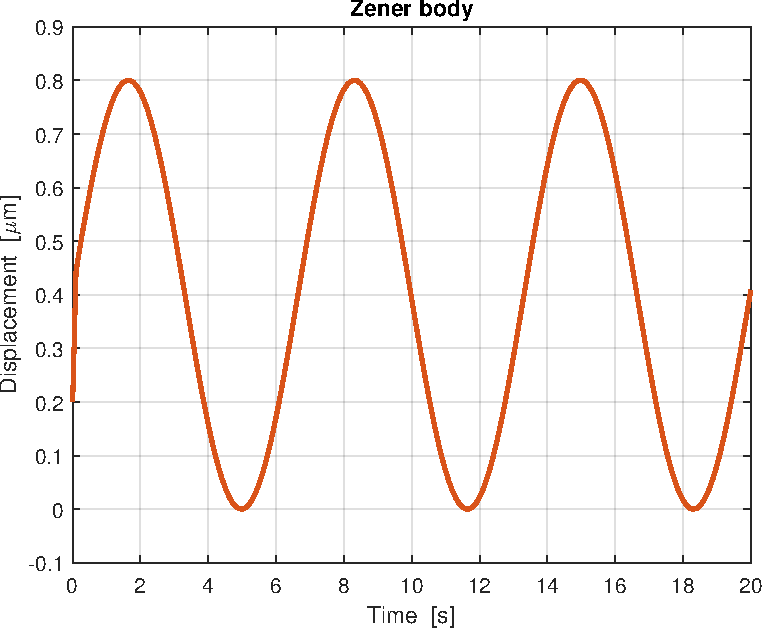
\includegraphics[width=0.95\linewidth]{../code/figs/harmonic_zener_}
		\caption{}
	\end{subfigure}\hfill
	\caption{Andamento dello spostamento dello smorzatore (sopra) e del corpo Zener (sotto) nel caso di ingresso a gradino (a,d); a onda quadra con periodo di 5s (b,e); sinusoide a frequenza 0.15 Hz (c,f).}
\end{figure*}

\subsection{Ingresso a gradino}




\textcolor{blue}{\lipsum[1-2]}

\subsection{Ingresso a onda quadra}




\textcolor{blue}{\lipsum[1-2]}

\subsection{Ingresso sinusoidale}




\textcolor{blue}{\lipsum[1-2]}



\section{Conclusioni}

\textcolor{blue}{\lipsum[1-2]}


\raggedbottom


\raggedbottom
\pagebreak
\section*{Disponiblità dei dati}

Il materiale è disponibile alla repository online del progetto: \url{https://github.com/mastroalex/ecm-mmt}.

\printbibliography[title=Riferimenti]
%\section*{References}

\clearpage
\onecolumn
\section*{Appendice}

